\documentclass[twoside]{book}

% Packages required by doxygen
\usepackage{calc}
\usepackage{doxygen}
\usepackage{graphicx}
\usepackage[utf8]{inputenc}
\usepackage{makeidx}
\usepackage{multicol}
\usepackage{multirow}
\usepackage{textcomp}
\usepackage[table]{xcolor}

% Font selection
\usepackage[T1]{fontenc}
\usepackage{mathptmx}
\usepackage[scaled=.90]{helvet}
\usepackage{courier}
\usepackage{amssymb}
\usepackage{sectsty}
\renewcommand{\familydefault}{\sfdefault}
\allsectionsfont{%
  \fontseries{bc}\selectfont%
  \color{darkgray}%
}
\renewcommand{\DoxyLabelFont}{%
  \fontseries{bc}\selectfont%
  \color{darkgray}%
}

% Page & text layout
\usepackage{geometry}
\geometry{%
  a4paper,%
  top=2.5cm,%
  bottom=2.5cm,%
  left=2.5cm,%
  right=2.5cm%
}
\tolerance=750
\hfuzz=15pt
\hbadness=750
\setlength{\emergencystretch}{15pt}
\setlength{\parindent}{0cm}
\setlength{\parskip}{0.2cm}
\makeatletter
\renewcommand{\paragraph}{%
  \@startsection{paragraph}{4}{0ex}{-1.0ex}{1.0ex}{%
    \normalfont\normalsize\bfseries\SS@parafont%
  }%
}
\renewcommand{\subparagraph}{%
  \@startsection{subparagraph}{5}{0ex}{-1.0ex}{1.0ex}{%
    \normalfont\normalsize\bfseries\SS@subparafont%
  }%
}
\makeatother

% Headers & footers
\usepackage{fancyhdr}
\pagestyle{fancyplain}
\fancyhead[LE]{\fancyplain{}{\bfseries\thepage}}
\fancyhead[CE]{\fancyplain{}{}}
\fancyhead[RE]{\fancyplain{}{\bfseries\leftmark}}
\fancyhead[LO]{\fancyplain{}{\bfseries\rightmark}}
\fancyhead[CO]{\fancyplain{}{}}
\fancyhead[RO]{\fancyplain{}{\bfseries\thepage}}
\fancyfoot[LE]{\fancyplain{}{}}
\fancyfoot[CE]{\fancyplain{}{}}
\fancyfoot[RE]{\fancyplain{}{\bfseries\scriptsize Generated on Fri Nov 29 2013 10:52:25 for Sodot by Doxygen }}
\fancyfoot[LO]{\fancyplain{}{\bfseries\scriptsize Generated on Fri Nov 29 2013 10:52:25 for Sodot by Doxygen }}
\fancyfoot[CO]{\fancyplain{}{}}
\fancyfoot[RO]{\fancyplain{}{}}
\renewcommand{\footrulewidth}{0.4pt}
\renewcommand{\chaptermark}[1]{%
  \markboth{#1}{}%
}
\renewcommand{\sectionmark}[1]{%
  \markright{\thesection\ #1}%
}

% Indices & bibliography
\usepackage{natbib}
\usepackage[titles]{tocloft}
\setcounter{tocdepth}{3}
\setcounter{secnumdepth}{5}
\makeindex

% Hyperlinks (required, but should be loaded last)
\usepackage{ifpdf}
\ifpdf
  \usepackage[pdftex,pagebackref=true]{hyperref}
\else
  \usepackage[ps2pdf,pagebackref=true]{hyperref}
\fi
\hypersetup{%
  colorlinks=true,%
  linkcolor=blue,%
  citecolor=blue,%
  unicode%
}

% Custom commands
\newcommand{\clearemptydoublepage}{%
  \newpage{\pagestyle{empty}\cleardoublepage}%
}


%===== C O N T E N T S =====

\begin{document}

% Titlepage & ToC
\hypersetup{pageanchor=false}
\pagenumbering{roman}
\begin{titlepage}
\vspace*{7cm}
\begin{center}%
{\Large Sodot \\[1ex]\large 0.\-9 }\\
\vspace*{1cm}
{\large Generated by Doxygen 1.8.4}\\
\vspace*{0.5cm}
{\small Fri Nov 29 2013 10:52:25}\\
\end{center}
\end{titlepage}
\clearemptydoublepage
\tableofcontents
\clearemptydoublepage
\pagenumbering{arabic}
\hypersetup{pageanchor=true}

%--- Begin generated contents ---
\chapter{Main Page}
\label{index}\hypertarget{index}{}Sodot is P\-H\-P application intended for allowing any user to post anonymous messages to any Facebook page.

\subsection*{settings.\-ini}

Copy the files into a any L\-A\-M\-P or W\-A\-M\-P server. Edit settings.\-ini located in the main directory. Fill in the following details\-:
\begin{DoxyItemize}
\item My\-S\-Q\-L username
\item My\-S\-Q\-L password
\item My\-S\-Q\-L database name
\item My\-S\-Q\-L table (You can just use the default)
\item My\-S\-Q\-L host (You can just use localhost if you don't know what is it)
\item Facebook page I\-D. You can find your Facebook page I\-D by going to this U\-R\-L\-: \href{http://graph.facebook.com/YOUR_FACEBOOK_PAGE_NAME}{\tt http\-://graph.\-facebook.\-com/\-Y\-O\-U\-R\-\_\-\-F\-A\-C\-E\-B\-O\-O\-K\-\_\-\-P\-A\-G\-E\-\_\-\-N\-A\-M\-E} and replace Y\-O\-U\-R\-\_\-\-F\-A\-C\-E\-B\-O\-O\-K\-\_\-\-P\-A\-G\-E\-\_\-\-N\-A\-M\-E with the name of the page or by using tools like \href{http://findmyfacebookid.com/}{\tt http\-://findmyfacebookid.\-com/}
\item The permanent Facebook access token of the application
\end{DoxyItemize}

\subsection*{Generating permanent Facebook Access Token}


\begin{DoxyItemize}
\item Create Facebook application and get the A\-P\-P K\-E\-Y.
\item \hyperlink{classInstall}{Install} the application on your page by going to \href{http://www.facebook.com/add.php?api_key={APP_KEY}&pages}{\tt http\-://www.\-facebook.\-com/add.\-php?api\-\_\-key=\{\-A\-P\-P\-\_\-\-K\-E\-Y\}\&pages} and replace the A\-P\-P\-\_\-\-K\-E\-Y with your Facebook application I\-D.
\item get the Access token by going to here\-: \href{https://developers.facebook.com/tools/explorer}{\tt https\-://developers.\-facebook.\-com/tools/explorer} and choose your Facebook application and generate the token.
\item verify it by going to \href{https://developers.facebook.com/tools/debug/access_token}{\tt https\-://developers.\-facebook.\-com/tools/debug/access\-\_\-token} paste the access token and see -\/expires\-: never.
\end{DoxyItemize}

\subsection*{\hyperlink{classInstall}{Install}}

After configuring the settings.\-ini, \hyperlink{classInstall}{Install} the program by going into /index.php?page=install

\subsection*{Use}

To use the application just go to root directory and write message. It should appear in your facebook page.

\subsection*{Test}

Sodot is using P\-H\-P\-Unit testing frameworl. in order to test it, just go to the test directory and type 'phpunit .'

\subsection*{Documentation}

Documentation is available at /documentation/html/

\subsection*{Regenerate doxygen}

Sodot is using Doxygen to auto document. for regenerating the documentation, go to the root directory and type 'doxygen Doxyfile'

\subsection*{T\-O\-D\-O\-:}


\begin{DoxyEnumerate}
\item Automate the F\-B application process.
\item Insert P\-H\-P testing. 
\end{DoxyEnumerate}
\chapter{Hierarchical Index}
\section{Class Hierarchy}
This inheritance list is sorted roughly, but not completely, alphabetically\-:\begin{DoxyCompactList}
\item \contentsline{section}{Controller}{\pageref{classController}}{}
\item \contentsline{section}{Install}{\pageref{classInstall}}{}
\item \contentsline{section}{Model}{\pageref{classModel}}{}
\item P\-D\-O\begin{DoxyCompactList}
\item \contentsline{section}{Database}{\pageref{classDatabase}}{}
\end{DoxyCompactList}
\item \contentsline{section}{Process\-\_\-post}{\pageref{classProcess__post}}{}
\item \contentsline{section}{Registry}{\pageref{classRegistry}}{}
\item \contentsline{section}{Send\-\_\-post}{\pageref{classSend__post}}{}
\item \contentsline{section}{Verification}{\pageref{classVerification}}{}
\end{DoxyCompactList}

\chapter{Class Index}
\section{Class List}
Here are the classes, structs, unions and interfaces with brief descriptions\-:\begin{DoxyCompactList}
\item\contentsline{section}{\hyperlink{classController}{Controller} \\*The controller of the application -\/ including router }{\pageref{classController}}{}
\item\contentsline{section}{\hyperlink{classDatabase}{Database} \\*D\-B functions -\/ extending P\-D\-O class }{\pageref{classDatabase}}{}
\item\contentsline{section}{\hyperlink{classInstall}{Install} \\*\hyperlink{classModel}{Model} that install the application on My\-S\-Q\-L }{\pageref{classInstall}}{}
\item\contentsline{section}{\hyperlink{classModel}{Model} \\*Loading all of the models }{\pageref{classModel}}{}
\item\contentsline{section}{\hyperlink{classProcess__post}{Process\-\_\-post} \\*Processing the initial content -\/ including verifying it and writing the logs }{\pageref{classProcess__post}}{}
\item\contentsline{section}{\hyperlink{classRegistry}{Registry} \\*Basic P\-H\-P based registry }{\pageref{classRegistry}}{}
\item\contentsline{section}{\hyperlink{classSend__post}{Send\-\_\-post} \\*Activating the Face\-Book A\-P\-I for sending the message to the F\-B page }{\pageref{classSend__post}}{}
\item\contentsline{section}{\hyperlink{classVerification}{Verification} \\*Including verfication functions }{\pageref{classVerification}}{}
\end{DoxyCompactList}

\chapter{File Index}
\section{File List}
Here is a list of all documented files with brief descriptions\-:\begin{DoxyCompactList}
\item\contentsline{section}{\hyperlink{index_8php}{index.\-php} }{\pageref{index_8php}}{}
\item\contentsline{section}{controller/\hyperlink{controller_8php}{controller.\-php} }{\pageref{controller_8php}}{}
\item\contentsline{section}{model/\hyperlink{database_8php}{database.\-php} }{\pageref{database_8php}}{}
\item\contentsline{section}{model/\hyperlink{install_8php}{install.\-php} }{\pageref{install_8php}}{}
\item\contentsline{section}{model/\hyperlink{model_8php}{model.\-php} }{\pageref{model_8php}}{}
\item\contentsline{section}{model/\hyperlink{process__post_8php}{process\-\_\-post.\-php} }{\pageref{process__post_8php}}{}
\item\contentsline{section}{model/\hyperlink{registry_8php}{registry.\-php} }{\pageref{registry_8php}}{}
\item\contentsline{section}{model/\hyperlink{send__post_8php}{send\-\_\-post.\-php} }{\pageref{send__post_8php}}{}
\item\contentsline{section}{model/\hyperlink{verification_8php}{verification.\-php} }{\pageref{verification_8php}}{}
\item\contentsline{section}{view/\hyperlink{main__page_8php}{main\-\_\-page.\-php} }{\pageref{main__page_8php}}{}
\end{DoxyCompactList}

\chapter{Class Documentation}
\hypertarget{classController}{\section{Controller Class Reference}
\label{classController}\index{Controller@{Controller}}
}


The controller of the application -\/ including router.  


\subsection*{Public Member Functions}
\begin{DoxyCompactItemize}
\item 
\hyperlink{classController_acd649140a4353af09a3a181ae5b00d2e}{\-\_\-\-\_\-construct} ()
\item 
\hyperlink{classController_a5cbb1ad733865bca5e76b52ecfbd8542}{invoke} ()
\end{DoxyCompactItemize}
\subsection*{Public Attributes}
\begin{DoxyCompactItemize}
\item 
\hyperlink{classController_a4078f8d070afa3d19a462422fa1a3547}{\$model}
\end{DoxyCompactItemize}


\subsection{Detailed Description}
The controller of the application -\/ including router. 

\subsection{Constructor \& Destructor Documentation}
\hypertarget{classController_acd649140a4353af09a3a181ae5b00d2e}{\index{Controller@{Controller}!\-\_\-\-\_\-construct@{\-\_\-\-\_\-construct}}
\index{\-\_\-\-\_\-construct@{\-\_\-\-\_\-construct}!Controller@{Controller}}
\subsubsection[{\-\_\-\-\_\-construct}]{\setlength{\rightskip}{0pt plus 5cm}Controller\-::\-\_\-\-\_\-construct (
\begin{DoxyParamCaption}
{}
\end{DoxyParamCaption}
)}}\label{classController_acd649140a4353af09a3a181ae5b00d2e}
Constructor of \hyperlink{classController}{Controller}. 

\subsection{Member Function Documentation}
\hypertarget{classController_a5cbb1ad733865bca5e76b52ecfbd8542}{\index{Controller@{Controller}!invoke@{invoke}}
\index{invoke@{invoke}!Controller@{Controller}}
\subsubsection[{invoke}]{\setlength{\rightskip}{0pt plus 5cm}Controller\-::invoke (
\begin{DoxyParamCaption}
{}
\end{DoxyParamCaption}
)}}\label{classController_a5cbb1ad733865bca5e76b52ecfbd8542}
The routing functions that decide which view to load. 

\subsection{Member Data Documentation}
\hypertarget{classController_a4078f8d070afa3d19a462422fa1a3547}{\index{Controller@{Controller}!\$model@{\$model}}
\index{\$model@{\$model}!Controller@{Controller}}
\subsubsection[{\$model}]{\setlength{\rightskip}{0pt plus 5cm}Controller\-::\$model}}\label{classController_a4078f8d070afa3d19a462422fa1a3547}
The model instance 

The documentation for this class was generated from the following file\-:\begin{DoxyCompactItemize}
\item 
controller/\hyperlink{controller_8php}{controller.\-php}\end{DoxyCompactItemize}

\hypertarget{classDatabase}{\section{Database Class Reference}
\label{classDatabase}\index{Database@{Database}}
}


D\-B functions -\/ extending P\-D\-O class.  


Inheritance diagram for Database\-:\begin{figure}[H]
\begin{center}
\leavevmode
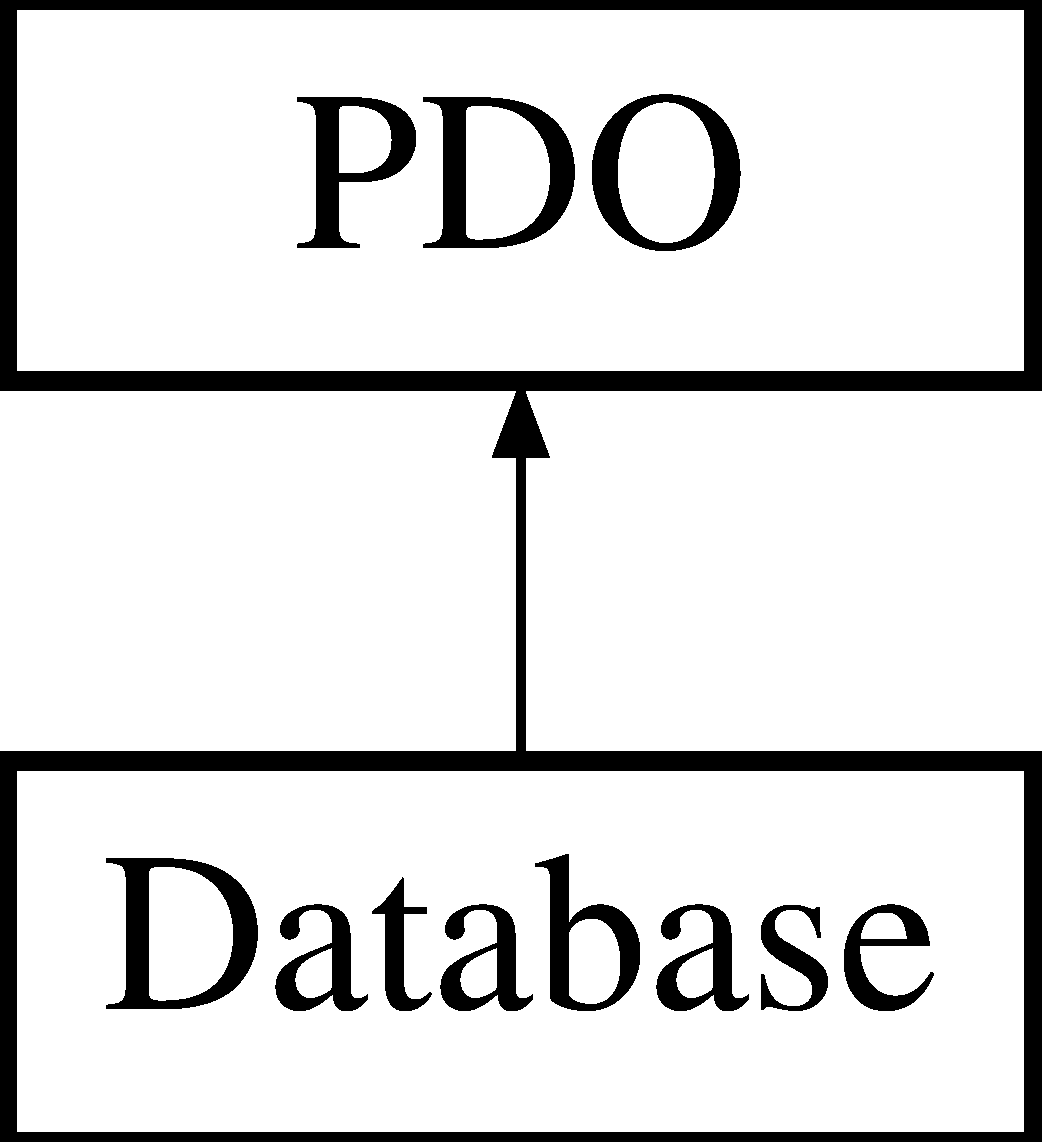
\includegraphics[height=2.000000cm]{classDatabase}
\end{center}
\end{figure}
\subsection*{Public Member Functions}
\begin{DoxyCompactItemize}
\item 
\hyperlink{classDatabase_abdd02ab861336df29f786db5368f7ff4}{check\-Table} (\$table)
\item 
\hyperlink{classDatabase_a8a449ab499e2c33437c78e12a0f8d91a}{write\-\_\-record} (\$array)
\end{DoxyCompactItemize}
\subsection*{Static Public Member Functions}
\begin{DoxyCompactItemize}
\item 
static \hyperlink{classDatabase_a8399325825e893103c463e644f817f86}{get\-Instance} ()
\end{DoxyCompactItemize}


\subsection{Detailed Description}
D\-B functions -\/ extending P\-D\-O class. 

\subsection{Member Function Documentation}
\hypertarget{classDatabase_abdd02ab861336df29f786db5368f7ff4}{\index{Database@{Database}!check\-Table@{check\-Table}}
\index{check\-Table@{check\-Table}!Database@{Database}}
\subsubsection[{check\-Table}]{\setlength{\rightskip}{0pt plus 5cm}Database\-::check\-Table (
\begin{DoxyParamCaption}
\item[{}]{\$table}
\end{DoxyParamCaption}
)}}\label{classDatabase_abdd02ab861336df29f786db5368f7ff4}
Check if table exist


\begin{DoxyParams}{Parameters}
{\em table} & The table name\\
\hline
\end{DoxyParams}
\begin{DoxyReturn}{Returns}
Tr\-U\-E if table exist, F\-A\-L\-S\-E if not. 
\end{DoxyReturn}
\hypertarget{classDatabase_a8399325825e893103c463e644f817f86}{\index{Database@{Database}!get\-Instance@{get\-Instance}}
\index{get\-Instance@{get\-Instance}!Database@{Database}}
\subsubsection[{get\-Instance}]{\setlength{\rightskip}{0pt plus 5cm}static Database\-::get\-Instance (
\begin{DoxyParamCaption}
{}
\end{DoxyParamCaption}
)\hspace{0.3cm}{\ttfamily [static]}}}\label{classDatabase_a8399325825e893103c463e644f817f86}
The constructor of the \hyperlink{classDatabase}{Database} singleton class \hypertarget{classDatabase_a8a449ab499e2c33437c78e12a0f8d91a}{\index{Database@{Database}!write\-\_\-record@{write\-\_\-record}}
\index{write\-\_\-record@{write\-\_\-record}!Database@{Database}}
\subsubsection[{write\-\_\-record}]{\setlength{\rightskip}{0pt plus 5cm}Database\-::write\-\_\-record (
\begin{DoxyParamCaption}
\item[{}]{\$array}
\end{DoxyParamCaption}
)}}\label{classDatabase_a8a449ab499e2c33437c78e12a0f8d91a}
Write arrays to table


\begin{DoxyParams}{Parameters}
{\em array} & The data in format of key =$>$ value\\
\hline
\end{DoxyParams}
\begin{DoxyReturn}{Returns}
The I\-D of the row inerted. 
\end{DoxyReturn}


The documentation for this class was generated from the following file\-:\begin{DoxyCompactItemize}
\item 
model/\hyperlink{database_8php}{database.\-php}\end{DoxyCompactItemize}

\hypertarget{classInstall}{\section{Install Class Reference}
\label{classInstall}\index{Install@{Install}}
}


\hyperlink{classModel}{Model} that install the application on My\-S\-Q\-L.  


\subsection*{Public Member Functions}
\begin{DoxyCompactItemize}
\item 
\hyperlink{classInstall_a35048e39db9649c7bc6e27569ae77bd3}{\-\_\-\-\_\-construct} ()
\item 
\hyperlink{classInstall_a377fcb5744e5f24dc471aad0105d4a26}{get\-Result} ()
\end{DoxyCompactItemize}


\subsection{Detailed Description}
\hyperlink{classModel}{Model} that install the application on My\-S\-Q\-L. 

\subsection{Constructor \& Destructor Documentation}
\hypertarget{classInstall_a35048e39db9649c7bc6e27569ae77bd3}{\index{Install@{Install}!\-\_\-\-\_\-construct@{\-\_\-\-\_\-construct}}
\index{\-\_\-\-\_\-construct@{\-\_\-\-\_\-construct}!Install@{Install}}
\subsubsection[{\-\_\-\-\_\-construct}]{\setlength{\rightskip}{0pt plus 5cm}Install\-::\-\_\-\-\_\-construct (
\begin{DoxyParamCaption}
{}
\end{DoxyParamCaption}
)}}\label{classInstall_a35048e39db9649c7bc6e27569ae77bd3}
Constructor of \hyperlink{classInstall}{Install} 

\subsection{Member Function Documentation}
\hypertarget{classInstall_a377fcb5744e5f24dc471aad0105d4a26}{\index{Install@{Install}!get\-Result@{get\-Result}}
\index{get\-Result@{get\-Result}!Install@{Install}}
\subsubsection[{get\-Result}]{\setlength{\rightskip}{0pt plus 5cm}Install\-::get\-Result (
\begin{DoxyParamCaption}
{}
\end{DoxyParamCaption}
)}}\label{classInstall_a377fcb5744e5f24dc471aad0105d4a26}
getting the result of the installation process. \begin{DoxyReturn}{Returns}
string to be displayed. 
\end{DoxyReturn}


The documentation for this class was generated from the following file\-:\begin{DoxyCompactItemize}
\item 
model/\hyperlink{install_8php}{install.\-php}\end{DoxyCompactItemize}

\hypertarget{classModel}{\section{Model Class Reference}
\label{classModel}\index{Model@{Model}}
}


Loading all of the models.  


\subsection*{Public Member Functions}
\begin{DoxyCompactItemize}
\item 
\hyperlink{classModel_af64f90f9a88a0eab985bcc89b32027a3}{process\-\_\-post} (\$post)
\end{DoxyCompactItemize}


\subsection{Detailed Description}
Loading all of the models. 

\subsection{Member Function Documentation}
\hypertarget{classModel_af64f90f9a88a0eab985bcc89b32027a3}{\index{Model@{Model}!process\-\_\-post@{process\-\_\-post}}
\index{process\-\_\-post@{process\-\_\-post}!Model@{Model}}
\subsubsection[{process\-\_\-post}]{\setlength{\rightskip}{0pt plus 5cm}Model\-::process\-\_\-post (
\begin{DoxyParamCaption}
\item[{}]{\$post}
\end{DoxyParamCaption}
)}}\label{classModel_af64f90f9a88a0eab985bcc89b32027a3}
Processing the post


\begin{DoxyParams}{Parameters}
{\em post} & the post array\\
\hline
\end{DoxyParams}
\begin{DoxyReturn}{Returns}
result array -\/ very similiar to post but include errors. no errors = everythink O\-K. 
\end{DoxyReturn}


The documentation for this class was generated from the following file\-:\begin{DoxyCompactItemize}
\item 
model/\hyperlink{model_8php}{model.\-php}\end{DoxyCompactItemize}

\hypertarget{classProcess__post}{\section{Process\-\_\-post Class Reference}
\label{classProcess__post}\index{Process\-\_\-post@{Process\-\_\-post}}
}


Processing the initial content -\/ including verifying it and writing the logs.  




\subsection{Detailed Description}
Processing the initial content -\/ including verifying it and writing the logs. 

The documentation for this class was generated from the following file\-:\begin{DoxyCompactItemize}
\item 
model/\hyperlink{process__post_8php}{process\-\_\-post.\-php}\end{DoxyCompactItemize}

\hypertarget{classRegistry}{\section{Registry Class Reference}
\label{classRegistry}\index{Registry@{Registry}}
}


Basic P\-H\-P based registry.  


\subsection*{Public Member Functions}
\begin{DoxyCompactItemize}
\item 
\hyperlink{classRegistry_a8692ca76b3f6d20e0233fdbdfa66f846}{\-\_\-\-\_\-construct} ()
\item 
\hyperlink{classRegistry_a68eb12ec266c565cde789cd0ff65a5bd}{\-\_\-\-\_\-set} (\$key, \$val)
\item 
\hyperlink{classRegistry_ae0c3afb597599f8d2cdf6f434533f6a2}{\-\_\-\-\_\-get} (\$key)
\end{DoxyCompactItemize}
\subsection*{Public Attributes}
\begin{DoxyCompactItemize}
\item 
\hyperlink{classRegistry_accb4d60e10b7d212a3097ab4c6d86a9d}{\$vars} = array()
\end{DoxyCompactItemize}


\subsection{Detailed Description}
Basic P\-H\-P based registry. 

\subsection{Constructor \& Destructor Documentation}
\hypertarget{classRegistry_a8692ca76b3f6d20e0233fdbdfa66f846}{\index{Registry@{Registry}!\-\_\-\-\_\-construct@{\-\_\-\-\_\-construct}}
\index{\-\_\-\-\_\-construct@{\-\_\-\-\_\-construct}!Registry@{Registry}}
\subsubsection[{\-\_\-\-\_\-construct}]{\setlength{\rightskip}{0pt plus 5cm}Registry\-::\-\_\-\-\_\-construct (
\begin{DoxyParamCaption}
{}
\end{DoxyParamCaption}
)}}\label{classRegistry_a8692ca76b3f6d20e0233fdbdfa66f846}
Constructor of \hyperlink{classRegistry}{Registry} 

\subsection{Member Function Documentation}
\hypertarget{classRegistry_ae0c3afb597599f8d2cdf6f434533f6a2}{\index{Registry@{Registry}!\-\_\-\-\_\-get@{\-\_\-\-\_\-get}}
\index{\-\_\-\-\_\-get@{\-\_\-\-\_\-get}!Registry@{Registry}}
\subsubsection[{\-\_\-\-\_\-get}]{\setlength{\rightskip}{0pt plus 5cm}Registry\-::\-\_\-\-\_\-get (
\begin{DoxyParamCaption}
\item[{}]{\$key}
\end{DoxyParamCaption}
)}}\label{classRegistry_ae0c3afb597599f8d2cdf6f434533f6a2}
Getter of registry item


\begin{DoxyParams}{Parameters}
{\em key} & The key of the item\\
\hline
\end{DoxyParams}
\begin{DoxyReturn}{Returns}
The value of the registry item. N\-U\-L\-L if not item was found. 
\end{DoxyReturn}
\hypertarget{classRegistry_a68eb12ec266c565cde789cd0ff65a5bd}{\index{Registry@{Registry}!\-\_\-\-\_\-set@{\-\_\-\-\_\-set}}
\index{\-\_\-\-\_\-set@{\-\_\-\-\_\-set}!Registry@{Registry}}
\subsubsection[{\-\_\-\-\_\-set}]{\setlength{\rightskip}{0pt plus 5cm}Registry\-::\-\_\-\-\_\-set (
\begin{DoxyParamCaption}
\item[{}]{\$key, }
\item[{}]{\$val}
\end{DoxyParamCaption}
)}}\label{classRegistry_a68eb12ec266c565cde789cd0ff65a5bd}
Setter of registry item


\begin{DoxyParams}{Parameters}
{\em key} & The key of the item \\
\hline
{\em val} & The value of the item \\
\hline
\end{DoxyParams}


\subsection{Member Data Documentation}
\hypertarget{classRegistry_accb4d60e10b7d212a3097ab4c6d86a9d}{\index{Registry@{Registry}!\$vars@{\$vars}}
\index{\$vars@{\$vars}!Registry@{Registry}}
\subsubsection[{\$vars}]{\setlength{\rightskip}{0pt plus 5cm}Registry\-::\$vars = array()}}\label{classRegistry_accb4d60e10b7d212a3097ab4c6d86a9d}
The variables of the registry 

The documentation for this class was generated from the following file\-:\begin{DoxyCompactItemize}
\item 
model/\hyperlink{registry_8php}{registry.\-php}\end{DoxyCompactItemize}

\hypertarget{classSend__post}{\section{Send\-\_\-post Class Reference}
\label{classSend__post}\index{Send\-\_\-post@{Send\-\_\-post}}
}


Activating the Face\-Book A\-P\-I for sending the message to the F\-B page.  




\subsection{Detailed Description}
Activating the Face\-Book A\-P\-I for sending the message to the F\-B page. 

The documentation for this class was generated from the following file\-:\begin{DoxyCompactItemize}
\item 
model/\hyperlink{send__post_8php}{send\-\_\-post.\-php}\end{DoxyCompactItemize}

\hypertarget{classVerification}{\section{Verification Class Reference}
\label{classVerification}\index{Verification@{Verification}}
}


Including verfication functions.  




\subsection{Detailed Description}
Including verfication functions. 

The documentation for this class was generated from the following file\-:\begin{DoxyCompactItemize}
\item 
model/\hyperlink{verification_8php}{verification.\-php}\end{DoxyCompactItemize}

\chapter{File Documentation}
\hypertarget{controller_8php}{\section{controller/controller.php File Reference}
\label{controller_8php}\index{controller/controller.\-php@{controller/controller.\-php}}
}
\subsection*{Classes}
\begin{DoxyCompactItemize}
\item 
class \hyperlink{classController}{Controller}
\begin{DoxyCompactList}\small\item\em The controller of the application -\/ including router. \end{DoxyCompactList}\end{DoxyCompactItemize}


\subsection{Detailed Description}
\hyperlink{classController}{Controller}

The controller of the application -\/ including router 
\hypertarget{index_8php}{\section{index.\-php File Reference}
\label{index_8php}\index{index.\-php@{index.\-php}}
}
\subsection*{Variables}
\begin{DoxyCompactItemize}
\item 
\hypertarget{index_8php_a388ef7b1db5e6f728e63cee704ce6e23}{{\bfseries \$controller} = new \hyperlink{classController}{Controller}()}\label{index_8php_a388ef7b1db5e6f728e63cee704ce6e23}

\end{DoxyCompactItemize}


\subsection{Detailed Description}
\hyperlink{index_8php}{index.\-php}

Calls the controller. 
\hypertarget{database_8php}{\section{model/database.php File Reference}
\label{database_8php}\index{model/database.\-php@{model/database.\-php}}
}
\subsection*{Classes}
\begin{DoxyCompactItemize}
\item 
class \hyperlink{classDatabase}{Database}
\begin{DoxyCompactList}\small\item\em D\-B functions -\/ extending P\-D\-O class. \end{DoxyCompactList}\end{DoxyCompactItemize}


\subsection{Detailed Description}
\hyperlink{classDatabase}{Database} Class

D\-B functions -\/ extending P\-D\-O class 
\hypertarget{install_8php}{\section{model/install.php File Reference}
\label{install_8php}\index{model/install.\-php@{model/install.\-php}}
}
\subsection*{Classes}
\begin{DoxyCompactItemize}
\item 
class \hyperlink{classInstall}{Install}
\begin{DoxyCompactList}\small\item\em \hyperlink{classModel}{Model} that install the application on My\-S\-Q\-L. \end{DoxyCompactList}\end{DoxyCompactItemize}


\subsection{Detailed Description}
\hyperlink{classInstall}{Install} model

\hyperlink{classModel}{Model} that install the application on My\-S\-Q\-L 
\hypertarget{model_8php}{\section{model/model.php File Reference}
\label{model_8php}\index{model/model.\-php@{model/model.\-php}}
}
\subsection*{Classes}
\begin{DoxyCompactItemize}
\item 
class \hyperlink{classModel}{Model}
\begin{DoxyCompactList}\small\item\em Loading all of the models. \end{DoxyCompactList}\end{DoxyCompactItemize}


\subsection{Detailed Description}
model main loader

Loading all of the models 
\hypertarget{process__post_8php}{\section{model/process\-\_\-post.php File Reference}
\label{process__post_8php}\index{model/process\-\_\-post.\-php@{model/process\-\_\-post.\-php}}
}
\subsection*{Functions}
\begin{DoxyCompactItemize}
\item 
\hyperlink{process__post_8php_a78331898e60f1bd282cea743a518705f}{\-\_\-\-\_\-construct} (\$post)
\item 
\hyperlink{process__post_8php_a1fdd68e1612712fe2ef591ee30bc1c0f}{get\-\_\-result} ()
\end{DoxyCompactItemize}
\subsection*{Variables}
\begin{DoxyCompactItemize}
\item 
Class {\bfseries Process\-\_\-post}
\item 
\hyperlink{process__post_8php_a79155f00a64b1dc5e717f64f53eb52a5}{\$db\-\_\-instance}
\item 
\hyperlink{process__post_8php_a531e4a386aaa7f3e06d3642dc38d7e80}{\$registry}
\item 
\hyperlink{process__post_8php_a112ef069ddc0454086e3d1e6d8d55d07}{\$result} = array()
\end{DoxyCompactItemize}


\subsection{Detailed Description}
Process post model

Processing the initial content -\/ including verifying it and writing the logs. 

\subsection{Function Documentation}
\hypertarget{process__post_8php_a78331898e60f1bd282cea743a518705f}{\index{process\-\_\-post.\-php@{process\-\_\-post.\-php}!\-\_\-\-\_\-construct@{\-\_\-\-\_\-construct}}
\index{\-\_\-\-\_\-construct@{\-\_\-\-\_\-construct}!process_post.php@{process\-\_\-post.\-php}}
\subsubsection[{\-\_\-\-\_\-construct}]{\setlength{\rightskip}{0pt plus 5cm}\-\_\-\-\_\-construct (
\begin{DoxyParamCaption}
\item[{}]{\$post}
\end{DoxyParamCaption}
)}}\label{process__post_8php_a78331898e60f1bd282cea743a518705f}
Constructor of \hyperlink{classProcess__post}{Process\-\_\-post}


\begin{DoxyParams}{Parameters}
{\em post} & Array that includes the post values. \\
\hline
\end{DoxyParams}
\hypertarget{process__post_8php_a1fdd68e1612712fe2ef591ee30bc1c0f}{\index{process\-\_\-post.\-php@{process\-\_\-post.\-php}!get\-\_\-result@{get\-\_\-result}}
\index{get\-\_\-result@{get\-\_\-result}!process_post.php@{process\-\_\-post.\-php}}
\subsubsection[{get\-\_\-result}]{\setlength{\rightskip}{0pt plus 5cm}get\-\_\-result (
\begin{DoxyParamCaption}
{}
\end{DoxyParamCaption}
)}}\label{process__post_8php_a1fdd68e1612712fe2ef591ee30bc1c0f}
getter if the result of the constructor 

\subsection{Variable Documentation}
\hypertarget{process__post_8php_a79155f00a64b1dc5e717f64f53eb52a5}{\index{process\-\_\-post.\-php@{process\-\_\-post.\-php}!\$db\-\_\-instance@{\$db\-\_\-instance}}
\index{\$db\-\_\-instance@{\$db\-\_\-instance}!process_post.php@{process\-\_\-post.\-php}}
\subsubsection[{\$db\-\_\-instance}]{\setlength{\rightskip}{0pt plus 5cm}\$db\-\_\-instance}}\label{process__post_8php_a79155f00a64b1dc5e717f64f53eb52a5}
The \hyperlink{classDatabase}{Database} instance \hypertarget{process__post_8php_a531e4a386aaa7f3e06d3642dc38d7e80}{\index{process\-\_\-post.\-php@{process\-\_\-post.\-php}!\$registry@{\$registry}}
\index{\$registry@{\$registry}!process_post.php@{process\-\_\-post.\-php}}
\subsubsection[{\$registry}]{\setlength{\rightskip}{0pt plus 5cm}\$registry}}\label{process__post_8php_a531e4a386aaa7f3e06d3642dc38d7e80}
The registry instance \hypertarget{process__post_8php_a112ef069ddc0454086e3d1e6d8d55d07}{\index{process\-\_\-post.\-php@{process\-\_\-post.\-php}!\$result@{\$result}}
\index{\$result@{\$result}!process_post.php@{process\-\_\-post.\-php}}
\subsubsection[{\$result}]{\setlength{\rightskip}{0pt plus 5cm}\$result = array()}}\label{process__post_8php_a112ef069ddc0454086e3d1e6d8d55d07}
The result of the process \hypertarget{process__post_8php_a4d6a7c0044f859bfec6c54966529e7d9}{\index{process\-\_\-post.\-php@{process\-\_\-post.\-php}!Process\-\_\-post@{Process\-\_\-post}}
\index{Process\-\_\-post@{Process\-\_\-post}!process_post.php@{process\-\_\-post.\-php}}
\subsubsection[{Process\-\_\-post}]{\setlength{\rightskip}{0pt plus 5cm}Class {\bf Process\-\_\-post}}}\label{process__post_8php_a4d6a7c0044f859bfec6c54966529e7d9}
{\bfseries Initial value\-:}
\begin{DoxyCode}
\{
    
    \textcolor{keyword}{public} \textcolor{keyword}{static} $post
\end{DoxyCode}

\hypertarget{registry_8php}{\section{model/registry.php File Reference}
\label{registry_8php}\index{model/registry.\-php@{model/registry.\-php}}
}
\subsection*{Classes}
\begin{DoxyCompactItemize}
\item 
class \hyperlink{classRegistry}{Registry}
\begin{DoxyCompactList}\small\item\em Basic P\-H\-P based registry. \end{DoxyCompactList}\end{DoxyCompactItemize}


\subsection{Detailed Description}
\hyperlink{classRegistry}{Registry} model

Basic P\-H\-P based registry 
\hypertarget{send__post_8php}{\section{model/send\-\_\-post.php File Reference}
\label{send__post_8php}\index{model/send\-\_\-post.\-php@{model/send\-\_\-post.\-php}}
}
\subsection*{Functions}
\begin{DoxyCompactItemize}
\item 
\hyperlink{send__post_8php_a7c00c6a4981f55404b49962a66b0746a}{\-\_\-\-\_\-construct} (\$\hyperlink{send__post_8php_aab26cf0bb1048ee920848ba27fa96168}{message})
\item 
\hyperlink{send__post_8php_aab26cf0bb1048ee920848ba27fa96168}{message} (\$data)
\end{DoxyCompactItemize}
\subsection*{Variables}
\begin{DoxyCompactItemize}
\item 
Class {\bfseries Send\-\_\-post}
\item 
\hyperlink{send__post_8php_a0690e3943aac124dbebc20bfb9419da3}{\$page\-\_\-id} = ''
\item 
\hyperlink{send__post_8php_a1cce3b6b968431b6802980fa6f949d13}{\$post\-\_\-url} = ''
\item 
\hyperlink{send__post_8php_a07610c5842cbcf4e9df3c0cc291ddc15}{\$page\-\_\-access\-\_\-token} = ''
\end{DoxyCompactItemize}


\subsection{Detailed Description}
Send post model

Activating the Face\-Book A\-P\-I for sending the message to the F\-B page 

\subsection{Function Documentation}
\hypertarget{send__post_8php_a7c00c6a4981f55404b49962a66b0746a}{\index{send\-\_\-post.\-php@{send\-\_\-post.\-php}!\-\_\-\-\_\-construct@{\-\_\-\-\_\-construct}}
\index{\-\_\-\-\_\-construct@{\-\_\-\-\_\-construct}!send_post.php@{send\-\_\-post.\-php}}
\subsubsection[{\-\_\-\-\_\-construct}]{\setlength{\rightskip}{0pt plus 5cm}\-\_\-\-\_\-construct (
\begin{DoxyParamCaption}
\item[{}]{\$message}
\end{DoxyParamCaption}
)}}\label{send__post_8php_a7c00c6a4981f55404b49962a66b0746a}
Constructor of \hyperlink{classSend__post}{Send\-\_\-post}


\begin{DoxyParams}{Parameters}
{\em message} & the message text \\
\hline
\end{DoxyParams}
\hypertarget{send__post_8php_aab26cf0bb1048ee920848ba27fa96168}{\index{send\-\_\-post.\-php@{send\-\_\-post.\-php}!message@{message}}
\index{message@{message}!send_post.php@{send\-\_\-post.\-php}}
\subsubsection[{message}]{\setlength{\rightskip}{0pt plus 5cm}message (
\begin{DoxyParamCaption}
\item[{}]{\$data}
\end{DoxyParamCaption}
)}}\label{send__post_8php_aab26cf0bb1048ee920848ba27fa96168}
Sending message with Face\-Book A\-P\-I and Curl


\begin{DoxyParams}{Parameters}
{\em data} & array, basicly including the content\\
\hline
\end{DoxyParams}
\begin{DoxyReturn}{Returns}
T\-R\-U\-E if success. 
\end{DoxyReturn}


\subsection{Variable Documentation}
\hypertarget{send__post_8php_a07610c5842cbcf4e9df3c0cc291ddc15}{\index{send\-\_\-post.\-php@{send\-\_\-post.\-php}!\$page\-\_\-access\-\_\-token@{\$page\-\_\-access\-\_\-token}}
\index{\$page\-\_\-access\-\_\-token@{\$page\-\_\-access\-\_\-token}!send_post.php@{send\-\_\-post.\-php}}
\subsubsection[{\$page\-\_\-access\-\_\-token}]{\setlength{\rightskip}{0pt plus 5cm}\$page\-\_\-access\-\_\-token = ''}}\label{send__post_8php_a07610c5842cbcf4e9df3c0cc291ddc15}
The page access token \hypertarget{send__post_8php_a0690e3943aac124dbebc20bfb9419da3}{\index{send\-\_\-post.\-php@{send\-\_\-post.\-php}!\$page\-\_\-id@{\$page\-\_\-id}}
\index{\$page\-\_\-id@{\$page\-\_\-id}!send_post.php@{send\-\_\-post.\-php}}
\subsubsection[{\$page\-\_\-id}]{\setlength{\rightskip}{0pt plus 5cm}\$page\-\_\-id = ''}}\label{send__post_8php_a0690e3943aac124dbebc20bfb9419da3}
The page id \hypertarget{send__post_8php_a1cce3b6b968431b6802980fa6f949d13}{\index{send\-\_\-post.\-php@{send\-\_\-post.\-php}!\$post\-\_\-url@{\$post\-\_\-url}}
\index{\$post\-\_\-url@{\$post\-\_\-url}!send_post.php@{send\-\_\-post.\-php}}
\subsubsection[{\$post\-\_\-url}]{\setlength{\rightskip}{0pt plus 5cm}\$post\-\_\-url = ''}}\label{send__post_8php_a1cce3b6b968431b6802980fa6f949d13}
The post url -\/ right now we are not using it \hypertarget{send__post_8php_a92ce328857a58124a9b4eedf35ae17b2}{\index{send\-\_\-post.\-php@{send\-\_\-post.\-php}!Send\-\_\-post@{Send\-\_\-post}}
\index{Send\-\_\-post@{Send\-\_\-post}!send_post.php@{send\-\_\-post.\-php}}
\subsubsection[{Send\-\_\-post}]{\setlength{\rightskip}{0pt plus 5cm}Class {\bf Send\-\_\-post}}}\label{send__post_8php_a92ce328857a58124a9b4eedf35ae17b2}
{\bfseries Initial value\-:}
\begin{DoxyCode}
\{
    
    \textcolor{keyword}{private} \hyperlink{process__post_8php_a531e4a386aaa7f3e06d3642dc38d7e80}{$registry}
\end{DoxyCode}

\hypertarget{verification_8php}{\section{model/verification.php File Reference}
\label{verification_8php}\index{model/verification.\-php@{model/verification.\-php}}
}
\subsection*{Functions}
\begin{DoxyCompactItemize}
\item 
\hyperlink{verification_8php_a3261c2319fbd5c6cef0851e7cdac806a}{\-\_\-\-\_\-construct} (\$post\-\_\-array)
\end{DoxyCompactItemize}
\subsection*{Variables}
\begin{DoxyCompactItemize}
\item 
Class {\bfseries Verification}
\item 
\hyperlink{verification_8php_a531e4a386aaa7f3e06d3642dc38d7e80}{\$registry}
\item 
\hyperlink{verification_8php_a112ef069ddc0454086e3d1e6d8d55d07}{\$result} = array()
\item 
\hyperlink{verification_8php_a90a4d28b2cb5de073936de187b621453}{\$error\-\_\-reasons}
\end{DoxyCompactItemize}


\subsection{Detailed Description}
\hyperlink{classVerification}{Verification} model

Including verfication functions. 

\subsection{Function Documentation}
\hypertarget{verification_8php_a3261c2319fbd5c6cef0851e7cdac806a}{\index{verification.\-php@{verification.\-php}!\-\_\-\-\_\-construct@{\-\_\-\-\_\-construct}}
\index{\-\_\-\-\_\-construct@{\-\_\-\-\_\-construct}!verification.php@{verification.\-php}}
\subsubsection[{\-\_\-\-\_\-construct}]{\setlength{\rightskip}{0pt plus 5cm}\-\_\-\-\_\-construct (
\begin{DoxyParamCaption}
\item[{}]{\$post\-\_\-array}
\end{DoxyParamCaption}
)}}\label{verification_8php_a3261c2319fbd5c6cef0851e7cdac806a}
Constructor of \hyperlink{classVerification}{Verification}


\begin{DoxyParams}{Parameters}
{\em post\-\_\-array} & Array that includes the post values.\\
\hline
\end{DoxyParams}
\begin{DoxyReturn}{Returns}
T\-R\-U\-E if everything O\-K. F\-A\-L\-S\-E if some verification function failed. 
\end{DoxyReturn}


\subsection{Variable Documentation}
\hypertarget{verification_8php_a90a4d28b2cb5de073936de187b621453}{\index{verification.\-php@{verification.\-php}!\$error\-\_\-reasons@{\$error\-\_\-reasons}}
\index{\$error\-\_\-reasons@{\$error\-\_\-reasons}!verification.php@{verification.\-php}}
\subsubsection[{\$error\-\_\-reasons}]{\setlength{\rightskip}{0pt plus 5cm}\$error\-\_\-reasons}}\label{verification_8php_a90a4d28b2cb5de073936de187b621453}
String that contains the reasons for error. \hypertarget{verification_8php_a531e4a386aaa7f3e06d3642dc38d7e80}{\index{verification.\-php@{verification.\-php}!\$registry@{\$registry}}
\index{\$registry@{\$registry}!verification.php@{verification.\-php}}
\subsubsection[{\$registry}]{\setlength{\rightskip}{0pt plus 5cm}\$registry}}\label{verification_8php_a531e4a386aaa7f3e06d3642dc38d7e80}
The registry instance \hypertarget{verification_8php_a112ef069ddc0454086e3d1e6d8d55d07}{\index{verification.\-php@{verification.\-php}!\$result@{\$result}}
\index{\$result@{\$result}!verification.php@{verification.\-php}}
\subsubsection[{\$result}]{\setlength{\rightskip}{0pt plus 5cm}\$result = array()}}\label{verification_8php_a112ef069ddc0454086e3d1e6d8d55d07}
The result array variable \hypertarget{verification_8php_ae087d6118933ecf9a05f114d6808b973}{\index{verification.\-php@{verification.\-php}!Verification@{Verification}}
\index{Verification@{Verification}!verification.php@{verification.\-php}}
\subsubsection[{Verification}]{\setlength{\rightskip}{0pt plus 5cm}Class {\bf Verification}}}\label{verification_8php_ae087d6118933ecf9a05f114d6808b973}
{\bfseries Initial value\-:}
\begin{DoxyCode}
\{
    
    \textcolor{keyword}{private} \hyperlink{process__post_8php_a79155f00a64b1dc5e717f64f53eb52a5}{$db\_instance}
\end{DoxyCode}

\hypertarget{main__page_8php}{\section{view/main\-\_\-page.php File Reference}
\label{main__page_8php}\index{view/main\-\_\-page.\-php@{view/main\-\_\-page.\-php}}
}
\subsection*{Variables}
\begin{DoxyCompactItemize}
\item 
\hypertarget{main__page_8php_a0a4baf0b22973c07685c3981f0d17fc4}{{\bfseries \$path} = dirname(\$\-\_\-\-S\-E\-R\-V\-E\-R\mbox{[}'P\-H\-P\-\_\-\-S\-E\-L\-F'\mbox{]}).'/view/'}\label{main__page_8php_a0a4baf0b22973c07685c3981f0d17fc4}

\item 
\hypertarget{main__page_8php_ac5267abe69bad3624bcb732c489d1f60}{if(isset(\$return\-\_\-message\-\_\-array)\&\&isset(\$return\-\_\-message\-\_\-array\mbox{[}'error'\mbox{]})) \\*
else if(isset(\$return\-\_\-message\-\_\-array)) \\*
print \$path print \$path print \\*
\$path if(isset(\$error)) {\bfseries endif}}\label{main__page_8php_ac5267abe69bad3624bcb732c489d1f60}

\item 
\hypertarget{main__page_8php_aa97e900a14ad42855f9688142e1e1552}{{\bfseries if} (isset(\$success))}\label{main__page_8php_aa97e900a14ad42855f9688142e1e1552}

\end{DoxyCompactItemize}


\subsection{Detailed Description}
Main page view

The main page view -\/ including the form and the output printing area. 
%--- End generated contents ---

% Index
\newpage
\phantomsection
\addcontentsline{toc}{part}{Index}
\printindex

\end{document}
